\documentclass[a4paper, amsfonts, amssymb, amsmath, reprint, showkeys, showpacs, nofootinbib, twoside]{revtex4-2}
\usepackage[english]{babel}
\usepackage[utf8]{inputenc}
\usepackage[colorinlistoftodos, color=green!40, prependcaption]{todonotes}
\usepackage{bm}% bold math
\usepackage{amsthm}
\usepackage{mathtools}
\usepackage{physics}
\usepackage{xcolor}
\usepackage{graphicx}
\usepackage[left=23mm,right=13mm,top=35mm,columnsep=15pt]{geometry} 
\usepackage{adjustbox}
\usepackage{placeins}
\usepackage[T1]{fontenc}
\usepackage{lipsum}
\usepackage{csquotes}
\usepackage[pdftex, pdftitle={Article}, pdfauthor={Author}]{hyperref} % For hyperlinks in the PDF
%\setlength{\marginparwidth}{2.5cm}
\bibliographystyle{apsrev4-2}
\hypersetup{
    colorlinks=true,
    linkcolor=blue,
    citecolor=blue,
    urlcolor=blue
}

\begin{document}
\title{Collective Behavior, Chemotaxis and Chirality in Active Matter: A Review}

\author{Yichen Lu$^{1,2}$}
\author{Zhigang Zheng$^{1,3,}$}
\email{Corresponding author. zgzheng@hqu.edu.cn}

\affiliation{ 
$^1$Institute of Systems Science, Huaqiao University, Xiamen 361021, China\\
$^2$School of Mathematical Sciences, Huaqiao University, Quanzhou, 362021, China\\
$^3$College of Information Science and Technology, Huaqiao University, Xiamen 361021, China
}

\date{\today} % Leave empty to omit a date

\begin{abstract}
    Active matter refers to a class of systems composed of self-propelled particles that can convert energy into motion and exhibit a variety of collective behaviors, such as flocking, swarming, and clustering. In this review, we focus on the collective behaviors of active matter, with a particular emphasis on the role of chemotaxis and chirality in shaping these behaviors. Chemotaxis is the ability of cells or organisms to move in response to chemical gradients in their environment, and it plays a crucial role in many biological processes, such as wound healing, immune response, and cancer metastasis. Chirality refers to the property of an object that is not superimposable on its mirror image, and it is a common feature of many biological systems, such as DNA, proteins, and cells. The combination of chemotaxis and chirality can lead to a wide range of interesting collective behaviors in active matter, such as phase separation, pattern formation, and dynamic self-assembly. We introduce the Keller--Segel and phoretic Brownian particle models of chemotactic active matter and discuss the role of chemotaxis in shaping the collective behaviors of active particles. We present the chiral active particle model and its extension and discuss the role of chirality in shaping the collective behaviors of active particles. Furthermore, we summarize the main findings of the review and discuss future research directions in the field of active matter.
\end{abstract}

\pacs{pacs}  % PACS, the Physics and Astronomy  % Classification Scheme.
\keywords{active matter, chemotaxis, chirality, collective behavior}

\maketitle

\section{\label{sec:introduction}Introduction}

Active matter represents a class of nonequilibrium systems composed of self-propelled particles that continuously convert energy into mechanical motion. This field has emerged as a vibrant area of interdisciplinary research, bridging physics, biology, materials science, and engineering. The collective behaviors exhibited by active matter systems—such as flocking in birds, schooling in fish, or clustering in synthetic colloids—demonstrate remarkable emergent properties that cannot be understood by simply examining individual components.

The study of active matter has revealed fundamental insights into nonequilibrium statistical physics while providing practical frameworks for designing bio-inspired materials and robotic swarms. This review systematically examines the current state of active matter research through four critical perspectives: modeling approaches, hydrodynamic theories, linear stability analyses, and data-driven methods for understanding swarming behaviors.

% \begin{figure*}
%     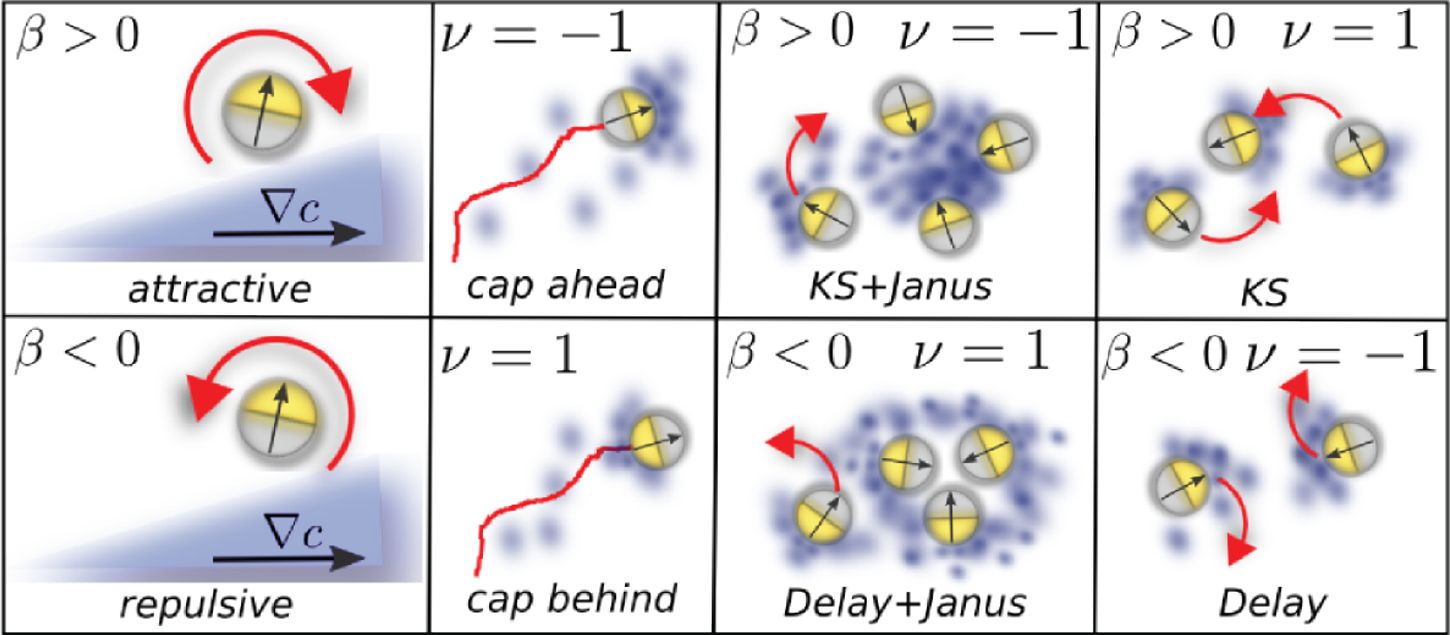
\includegraphics[width=0.7\textwidth]{./figs/schematicPlot1.png}
%     \caption{
%         \label{fig:schematicPlot1} Schematic plot of the chemotactic response of active particles to a chemo-attractant. Here, KS represents the Keller--Segel instability, and Janus and Delay stand for the Janus instability and the delay induced instability discussed in the text. Reproduced with permission from ref.~\cite{PhysRevLett.118.268001}. Copyright 2017 American Physical Society.
%     }
% \end{figure*}

\section{\label{sec:models}Modeling Approaches in Active Matter}

The theoretical foundation of active matter systems begins with particle-based models that capture the essential features of self-propelled particles and their interactions. Several paradigmatic models have emerged as standard frameworks for studying active matter phenomena.

\subsection{Vicsek Model and Its Variants}

The Vicsek model (Vicsek et al., 1995) represents one of the simplest yet most influential models for collective motion. It describes point particles moving at constant speed that align their directions of motion with neighbors within a fixed interaction radius. The model's dynamics are governed by:
\begin{subequations}
    \label{eq:agentsChemotaxis}
    \begin{align}
        \mathbf{x}_i\left( t+1 \right) &=\mathbf{x}_i\left( t \right) +\mathbf{v}_i\left( t \right) \Delta t\;,
        \\
        \theta_i \left( t+1 \right) &=\langle \theta \left( t \right) \rangle _r+\Delta \theta_i \;,
    \end{align}
\end{subequations}
where $\mathbf{x}_i$ is the position of particle $i$, $\mathbf{v}_i$ is its velocity, $\Delta t$ is the time step, $\theta_i$ is the orientation of particle $i$, $\langle \theta \left( t \right) \rangle _r$ is the average orientation of neighbors within a radius $r$, and $\Delta \theta_i$ is a random perturbation to account for noise. The Vicsek model has been extended to include various interactions, such as repulsion, attraction, and alignment, leading to rich phase diagrams and emergent behaviors.

\begin{figure}
    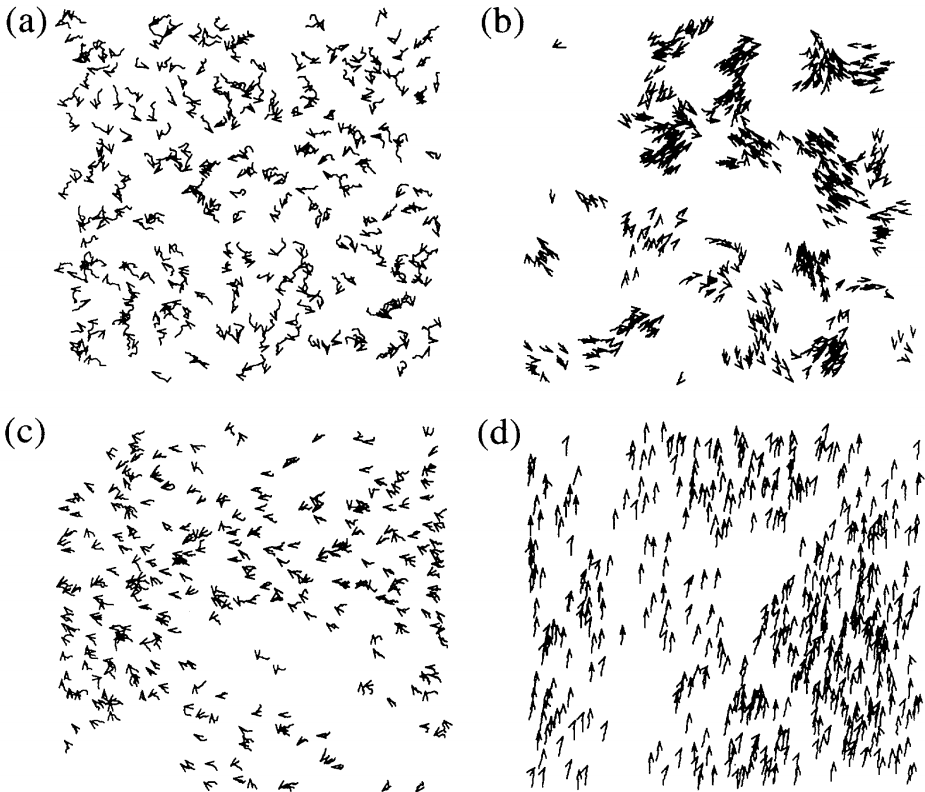
\includegraphics[width=0.49\textwidth]{./figs/vicsekSnapshots.png}
    \caption{
        \label{fig:vicsekSnapshots}
        In this figure the velocities of the particles are displayed for varying values of the density and the noise.
        The actual velocity of a particle is indicated by a small arrow, while their trajectory for the last 20 time steps is shown by a short continuous curve. he number of particles is $N = 300$ in each case. Copyright 2017 American Physical Society.
    }
\end{figure}



\begin{acknowledgments}
This work is partially supported by The Nonlinear Dynamics Research Group led by Professor Zheng and Institute of Systems Science, Huaqiao University, Xiamen.
\end{acknowledgments}

\bibliography{ref}

\end{document}
